% ****** Start of file apssamp.tex ******
%
%   This file is part of the APS files in the REVTeX 4.2 distribution.
%   Version 4.2a of REVTeX, December 2014
%
%   Copyright (c) 2014 The American Physical Society.
%
%   See the REVTeX 4 README file for restrictions and more information.
%
% TeX'ing this file requires that you have AMS-LaTeX 2.0 installed
% as well as the rest of the prerequisites for REVTeX 4.2
%
% See the REVTeX 4 README file
% It also requires running BibTeX. The commands are as follows:
%
%  1)  latex apssamp.tex
%  2)  bibtex apssamp
%  3)  latex apssamp.tex
%  4)  latex apssamp.tex
%
\documentclass[%
 reprint,
%superscriptaddress,
%groupedaddress,
%unsortedaddress,
%runinaddress,
%frontmatterverbose, 
%preprint,
%preprintnumbers,
%nofootinbib,
%nobibnotes,
%bibnotes,
 amsmath,amssymb,
 aps,
%pra,
%prb,
%rmp,
%prstab,
%prstper,
%floatfix,
]{revtex4-2}

\usepackage{graphicx}% Include figure files
\usepackage{dcolumn}% Align table columns on decimal point
\usepackage{bm}% bold math
\usepackage{kotex} % Korean
\usepackage{amsmath}
\usepackage{mathrsfs}
\usepackage{physics}
% \usepackage{fontspec}
% \usepackage{unicode-math}

%\usepackage{hyperref}% add hypertext capabilities
%\usepackage[mathlines]{lineno}% Enable numbering of text and display math
%\linenumbers\relax % Commence numbering lines

%\usepackage[showframe,%Uncomment any one of the following lines to test 
%%scale=0.7, marginratio={1:1, 2:3}, ignoreall,% default settings
%%text={7in,10in},centering,
%%margin=1.5in,
%%total={6.5in,8.75in}, top=1.2in, left=0.9in, includefoot,
%%height=10in,a5paper,hmargin={3cm,0.8in},
%]{geometry}

\begin{document}

\preprint{APS/123-QED}

% \title{Manuscript Title:\\with Forced Linebreak}% Force line breaks with \\
\title{Coupling exponents of three-state Potts model on two dimensional square lattice
}
% \thanks{A footnote to the article title}%

\author{SungBin LEE (이성빈, 李誠彬)}
\email{rqtoe@snu.ac.kr}
\affiliation{Department of Physics and Astronomy, Seoul National University, \\
1, Gwanak-ro, Gwank-gu, Seoul, Republic of Korea, 08826}

% \author{Second Author}%
% \email{Second.Author@institution.edu}
% \affiliation{%
% Authors' institution and/or address\\
% This line break forced with \textbackslash\textbackslash
% }%

% \collaboration{MUSO Collaboration}%\noaffiliation

% \author{Charlie Author}
% \homepage{http://www.Second.institution.edu/~Charlie.Author}
% \affiliation{
%  Second institution and/or address\\
%  This line break forced% with \\
% }%
% \affiliation{
%  Third institution, the second for Charlie Author
% }%
% \author{Delta Author}
% \affiliation{%
% Authors' institution and/or address\\
% This line break forced with \textbackslash\textbackslash
% }%

% \collaboration{CLEO Collaboration}%\noaffiliation

\date{\today}% It is always \today, today,
%  but any date may be explicitly specified

\begin{abstract}
The key idea behind studying critical behavior of physical systems with phase transition 
is determining their critical exponents respective to the coupling parameters, both 
numerically and theoretically. In a numerical aspect, methods like Finite Size Scaling and 
Monte Carlo Renormalization Group is utilized to characterize those universal parameters 
while we can also apply Real-Space Renormalization Group and Conformal Field Theory to 
directly calculate the exponents. Here we explicitly derive a critical exponent for the 
three-state Potts Model in two dimensional square lattice, and compare the numerical and 
theoretical results with the known value. We concluded that both Finite Size Scaling and 
Real-Space Renormalization Group shows an accurate results within a reasonable margin. 
\begin{description}
% \item[Usage]
% Secondary publications and information retrieval purposes.
% \item[Structure]
% You may use the \texttt{description} environment to structure your abstract;
% use the optional argument of the \verb+\item+ command to give the category of each item. 
\item[Keywords]
Renormalization Group, 3-state Potts model, Critical Exponents, Universality Class
\end{description}
\end{abstract}

\maketitle

%\tableofcontents

% \section{\label{sec:intro}Introduction}

\section{\label{sec:potts}3-state 2D Potts Model}
As a generalization of the Ising model, the Potts model named after Renfrey Potts, is a 
physical system of interacting spins on a crystalline lattice which shows phase transition 
with ferromagnetic phase. It can be generalized into several other important models in 
statistical physics, with examples being, but not limited to, the XY model, the Heisenberg 
Model, and the N-vector model. \\

The Potts model consists of discrete spins that are placed on a lattice. In this study, 
we will only consider two-dimensional square Euclidean lattice with continuous boundary 
condition. \\

The classical Hamiltonian for this model can be written by a combination of coupling 
parameters and spins.

\begin{eqnarray}
\mathcal{H} = -\mathcal{K} \sum_{\left<i,j\right>} \delta(s_{i}, s_{j}) - h \sum_{i} 
\delta(s_{i},s_{ghost}) \label{ham}
\end{eqnarray}

While $s_{i}$ is a spin respective to the location $i$ on lattice with value from $0$ to 
$q-1$ for q-state Potts model. $\mathcal{K}$ and $h$ represents the coupling parameters 
in association with the spin and external field, respectively. In this paper, we will 
assume $s_{ghost}$; a spin interacting with an external field, to be $0$ without losing 
generality. \\

As a result, the partition function and bulk free energy density for such system is 
given as

\begin{eqnarray}
\mathcal{Z} = \sum_{\{s_{i}\}} \exp \left[{\mathcal{K}}\sum_{\left<i,j\right>}
\delta(s_{i},s_{j}) + h \sum_{i} \delta(s_{i},0)\right] \label{par}
\end{eqnarray}

\begin{eqnarray}
f_{bulk} = f := - \lim_{V \rightarrow \infty} \left[\frac{\ln \mathcal{Z}}{V}
\right] \label{free}
\end{eqnarray}

It is known that the q-state Potts model on 2D square lattice has a critical fixed point 
on the following basis.

\begin{eqnarray}
\left(\mathcal{K}_{c}, h_{c} \right) = \left(1 / T_{c}, h_{c}\right) = 
\left(\ln[1+\sqrt q], 0 \right) \label{cfp}
\end{eqnarray}

Eq.~(\ref{cfp}) can be easily proven based on a duality relation between two coupling 
parameter $\mathcal{K}$ and $\mathcal{K}^{*}$ on 2D square lattice: 
$\mathcal{K} = \mathcal{K}^{*} = \mathcal{K}_{c}$ is satisfied on a critical fixed point

\begin{eqnarray}
e^{-\mathcal{K}^{*}} = \frac{e^{\mathcal{K}} - 1}{e^{\mathcal{K}} + q - 1}
\end{eqnarray}

Note that the standard ferromagnetic Potts model in 2d shows continuous phase transition 
for $1 \leq q \leq 4$ and first-order phase transition for $q>4$. In this research, we 
will only consider cases where $q$ is $3$.\\

Following the definition of Hamiltonian in Eq.~(\ref{ham}), we determine the order 
parameter $m$ to be

\begin{eqnarray}
m = \frac{q \rho - 1}{q - 1} \text{, where } \rho = \frac{1}{V} \sum_{i} 
\delta(s_{i},0) \label{order}
\end{eqnarray}

and correlation function $G(i,j)$ and correlation length $\xi(T)$ of the system to be

\begin{widetext}
\begin{eqnarray}
G(i,j) = \left<\frac{q \delta(s_{i}, s_{j}) - 1}{q - 1}\right> - \left<\frac{q 
\delta(s_{i}, 0) - 1}{q - 1}\right> \left<\frac{q \delta(s_{j}, 0) - 1}{q - 1}\right> 
\propto \frac{1}{|i-j|^{d-2+\eta}} \exp \left[-\frac{|i-j|}{\xi(T)}\right] \label{corr}
\end{eqnarray}
\end{widetext}

It is straight forward to prove that correlation function is $0$ for both completely 
ordered and dis-ordered phases.

\section{\label{sec:scaling} Critical Exponents and Scaling Relations}

The basic approach to quantitatively analyzing the system in statistical physics is 
to follow the variation of physical quantities as we increase the length scale. Such 
approach is known as coarse graining and rescaling, which allows us to systematically 
take into account fluctuations near the critical point by tracing out short-range 
fluctuations and shift our attention to longer-length behavior of the system. \\

The basis of coarse graining and rescaling analysis is the rule that the partition 
function is invariant.

\begin{gather}
\mathcal{Z}(\mathcal{H}) = \sum_{s'}\sum_{s}e^{-\mathcal{H}} = \sum_{s'}
e^{-\mathcal{H}'} = \mathcal{Z}'\left(\mathcal{H}'\right) \label{parequal}\\
\text{where } e^{-\mathcal{H}'} = \sum_{s} e^{-\mathcal{H}} \leftrightarrow 
\mathcal{H}' = - \ln \left[\sum_{s} e^{-\mathcal{H}}\right] \label{eqn:newHam}
\end{gather}


Combining Eqs.~(\ref{free}) and~(\ref{parequal}), the bulk free energy density of 
the system changes as we rescale the system with scale factor $b > 1$.

\begin{eqnarray}
f(\mathcal{K}) = b^{-d}f(\mathcal{K}') \label{fund1}
\end{eqnarray}

Eq.~(\ref{fund1}) is known as the fundamental relation in thermodynamics and statistical 
physics. For $\mathcal{K}$ consisting of nearest-neighbor coupling and external magnetic 
field, we arrive at

\begin{eqnarray}
f(t,h) = b^{-d}f(b^{y_{t}}t, b^{y_{h}}h) \text{, where } t = \frac{T-T_{c}}{T_{c}} 
\label{fund2}
\end{eqnarray}

Where $y_{t}$ and $y_{h}$ are the thermal and magnetic coupling exponents, respectively.
It is worth noting that Eq.~(\ref{fund2}) leads to several important scaling relations 
in critical phenomena. \\

The degree of singularity of physical quantities near the critical point is described 
by the critical exponents defined below, note that each exponents represents the asymptotic 
behavior of each physical quantities as the system reaches criticality.

\begin{widetext}
\begin{gather}
\lim_{t \rightarrow 0} C_{v} \propto |t|^{-\alpha} \text{, where } C_{v} := 
-T \frac{\partial^{2} f(t,h)}{\partial t^{2}}\bigg|_{h=0} \text{ is a Specific Heat} 
\label{alpha} \\
\lim_{t \rightarrow 0-} M(h=0) \propto (-t)^{\beta} \text{, where } M := 
- \frac{\partial f(t,h)}{\partial h} \text{ is a Order Parameter} \label{beta} \\
\lim_{t \rightarrow 0} X_{T} \propto |t|^{-\gamma} \text{, where } X_{T} := 
-\frac{\partial^{2} f(t,h)}{\partial h^{2}}\bigg|_{h=0} \text{ is a Susceptibility} 
\label{gamma} \\
\lim_{h \rightarrow 0} M(t=0) \propto |h|^{1/\delta} \label{delta} \\
\lim_{t \rightarrow 0} \xi(t) \propto |t|^{-\nu} \label{nu} \\
\lim_{t \rightarrow 0} G(i,j) \propto \frac{1}{|i-j|^{d-2+\eta}} 
\text{, where } d \text{ and } \eta \text{ is a dimension and an anomalous dimension, 
respectively} \label{eta}
\end{gather}
\end{widetext}

Combining Eq.~(\ref{fund2}) with Eqs.~(\ref{alpha}) to~(\ref{delta}), we can determine 
the critical exponents $\alpha \text{, } \beta \text{, } \gamma \text{, and } \delta$ as 
follows:

\begin{gather}
-\alpha y_{t} + 2y_{t} - d = 0 \rightarrow \alpha = 2-d/y_{t} \\
\beta y_{t} + y_{h} - d = 0 \rightarrow \beta = (d-y_{h})/y_{t} \\
-\gamma y_{t} + 2y_{h} - d = 0 \rightarrow \gamma = (2y_{h}-d)/y_{t} \\
y_{h} / \delta + y_{h} - d = 0 \rightarrow \delta = y_{h}/(d-y_{h})
\end{gather}

One can also derive the relations for $\nu \text{ and } \eta$ by applying 
fluctuation-dissipation theorem and a trivial scaling relation for correlation length
$\xi(t) = b\xi(tb^{y_{t}})$, please refer to Appendix~\ref{appx:fluc} for further 
details regarding the relationship between the correlation function and susceptibility.

\begin{gather}
-\nu y_{t} + (2y_{h} - d)/(2 - \eta) = 0 \rightarrow \nu = 1/y_{t} \\
(2y_{h} - d)/(2 - \eta) = 1 \rightarrow \eta = d-2y_{h}+2
\end{gather}

% It is straight forward to show that Rushbrooke's equality is satisfied.

% \begin{eqnarray}
% \alpha + 2\beta + \gamma = 2
% \end{eqnarray}

\section{\label{sec:fss}Numerical Method 1: \\ Finite Size Scaling}
\subsection{Monte Carlo Simulation and Heat-Bath Method}
Monte Carlo simulations are realized as the numerical implementation of stochastic 
dynamics represented by the master equation, which describes how the set of probabilities 
evolves with time. \\

For spin configuration $a = \{s_{1}, s_{2}, ... s_{N}\}$, let us denote the state of a
system using a probability that the system has a configuration $a$ at time $t, P(a,t)$.
For the ising model, the total number of possible configuration $a$ is $2^N$ while 
for $q$-state Potts model, it is $q^N$.
Suppose that the configuration changes from a to b with the transition probability 
$w(a \rightarrow b)\Delta t$ in a small time interval $\Delta t$. The net change of the 
probability for the system in configuration $a$ should satisfy the following master equation.

\begin{widetext}
\begin{eqnarray}
P(a,t+\Delta t) - P(a, t) = -\sum_{b \ne a} w(a \rightarrow b) P(a,t) \Delta t + 
\sum_{b \ne a} w(b \rightarrow a) P(b,t) \Delta t \label{master}
\end{eqnarray}
\end{widetext}

It is critical to choose appropriate transition probabiltiles in Monte Carlo simulations 
so that the equilibrium distribution is of the Gibbs-Boltzmann form $P(a,t) = e^{-H(a)}/
\mathcal{Z}:=P_{eq}(a)$. Suppose that an equilibrium has been achieved in the master 
equation Eq.~(\ref{master}) with $P(a,t) = P_{eq}(a)$. Then, the left-hand side vanishes and consequently

\begin{eqnarray}
\sum_{b \ne a} w(a \rightarrow b) P_{eq}(a) = \sum_{b \ne a} w(b \rightarrow a) P_{eq}(b)
\end{eqnarray}

A sufficient condition for the above relation to hold is to equate both sides term by term,

\begin{gather}
w(a \rightarrow b) P_{eq}(a) = w(b \rightarrow a) P_{eq}(b) \\
\frac{w(a \rightarrow b)}{w(b \rightarrow a)} = e^{-\beta \left[H(b) - H(a)\right]} \label{balcond}
\end{gather}

This relation is called the detailed balance condition that the transition probability 
should satisfy. A common choide of the transition probability that satisfied such condition
is a Heat-Bath method described below.

\begin{eqnarray}
w(a \rightarrow b) = \frac{e^{-\beta H(b)}}{e^{-\beta H(a)} + e^{-\beta H(b)}} \label{heat-bath}
\end{eqnarray}

Note that in Monte Carlo simulations one regards the calculation of the expectation valule 
of a physical quantity $O$ as an average over the configurations generated by the stochastic 
dynamics.

\subsection{Finite Size Scaling}
To extract coupling exponents from numerical data, we would have to run simulations 
where critical phenomena take place in macroscopic system. We can, however, carry out 
numerical computations only for finite-size systems. Therefore, it is not possible for 
our physical quantities to show authentic singular behavior since critical phenomena 
only happens at the thermodynamic limit, i.e. either when system size it infinite or 
the temperature is zero.\\ 

Since the parameter should be carefuly tuned for the system to reach the critical point, 
we should include the inverse of system size $L^{-1}$ in the argument of free energy 
density. 

\begin{eqnarray}
f(t,h,L^{-1}) = b^{-d}f(b^{y_{t}}t, b^{y_{h}}h, bL^{-1}) \label{rev-fund}
\end{eqnarray}

If we combine Eq.~(\ref{rev-fund}) with the definition described in Eq.~(\ref{alpha}),
~(\ref{beta}), and~(\ref{gamma}), we obtain

\begin{gather}
C_{v}(t,0,L^{-1}) = b^{2y_{t}-d}\partial_{t}^{2}f(b^{y_{t}}t,0,bL^{-1}) \\
m(t,h,L^{-1}) = b^{y_{h}-d}\partial_{h}f(b^{y_{t}}t,b^{y_{h}}h,bL^{-1}) \\
X_{T}(t,0,L^{-1}) = b^{2y_{h}-d}\partial_{h}^{2}f(b^{y_{t}}t,0,bL^{-1})
\end{gather}

If we insert $b=L$ and rewrite the equation,

\begin{gather}
L^{d-2y_{t}}C_{v}(t,L^{-1}) = \Phi_{1}(L^{y_{t}}t) \label{cv} \\
L^{d-y_{h}}m(t,L^{-1}) = \Phi_{2}(L^{y_{t}}t) \label{m1} \\
L^{d-y_{h}}m(h,L^{-1}) = \Phi_{3}(L^{y_{h}}h) \label{m2} \\
L^{d-2y_{h}}X_{T}(t,L^{-1}) = \Phi_{4}(L^{y_{t}}t) \label{xt}
\end{gather}

Therefore, we can estimate the exact value of coupling exponents by plotting physical 
quantities on graph with appropriate x and y axis in respective to Eqs.~(\ref{cv}) 
to~(\ref{xt}). \\

The result of the numerical computation is displayed from Fig.~\ref{fig:binder} to
~\ref{fig:corrfunc}, each containing a corresponding physical quantities introduced 
in Section~\ref{sec:scaling}. In general, the critical exponents that forms the 
universality class of 3-state 2D Potts Model coincides with the numerical data generated 
by Monte Carlo simulations, refer to Table~\ref{tab:universality} in 
Appendix~\ref{appx:universal} for the full list of critical exponents.

\begin{figure*}[b]
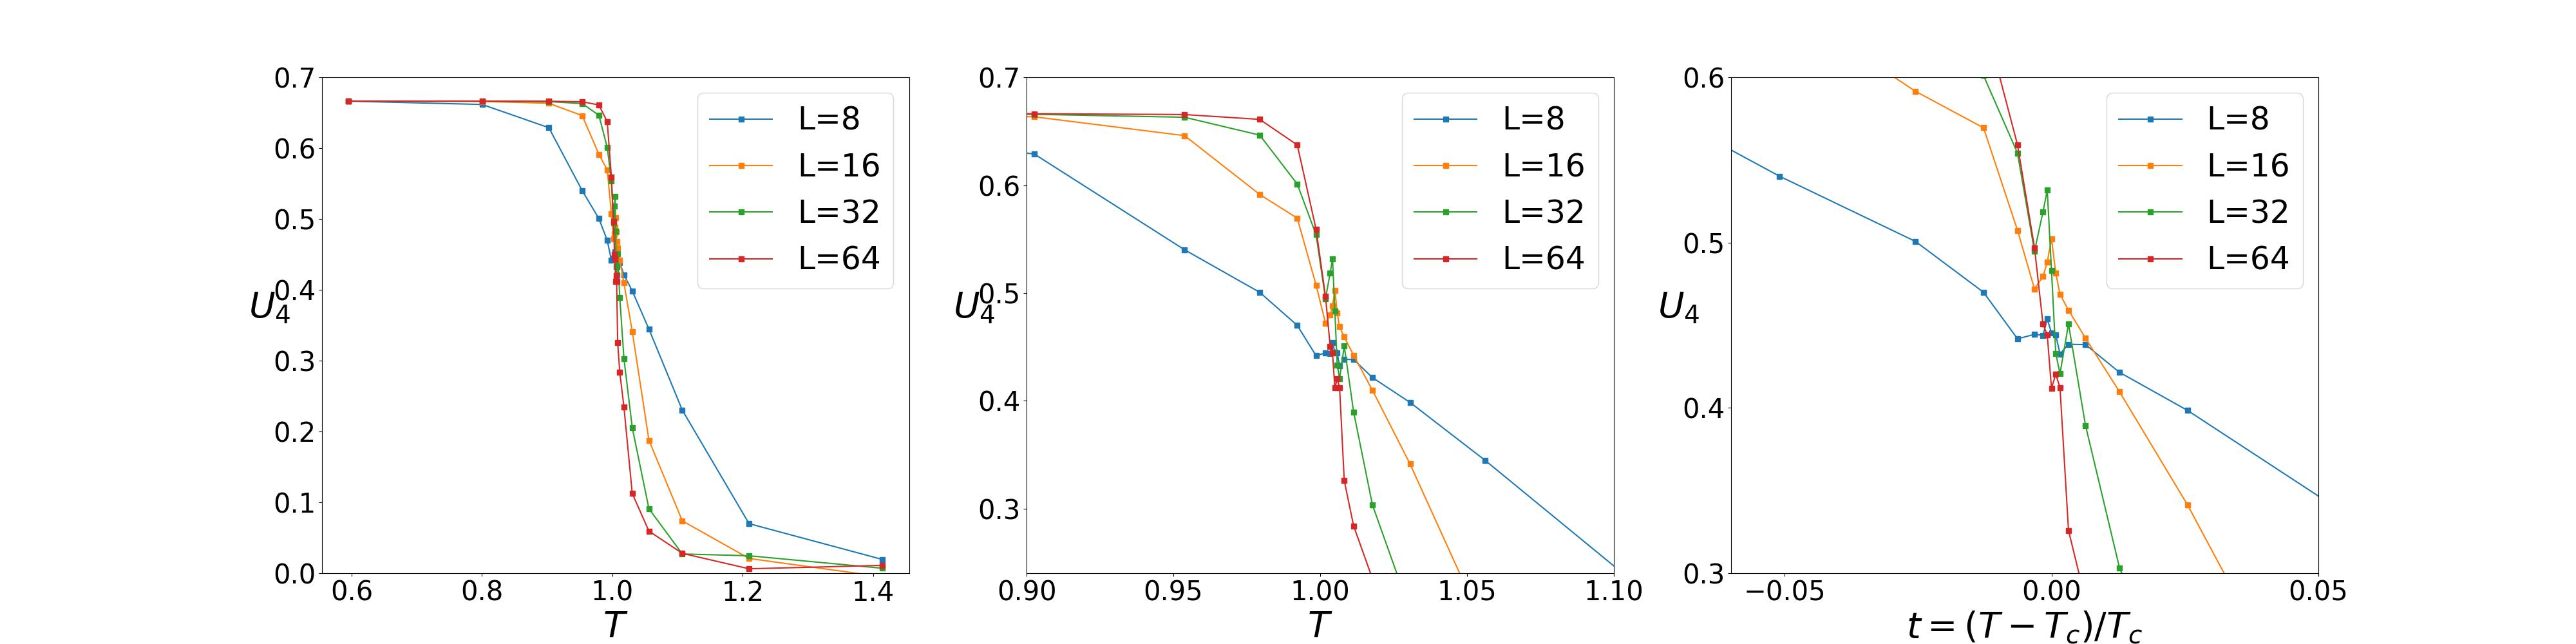
\includegraphics[width=1\textwidth]{../fig/Binder Cumulant (3-state 2D Potts).jpg}
\caption{\label{fig:binder} Binder Cumulant $U_{4}$ of the system at Size = 8, 16, 32, 
and 64. The $T_{c}$ where the cumulant intersect is 1.005.}
\end{figure*}

\begin{figure*}[b]
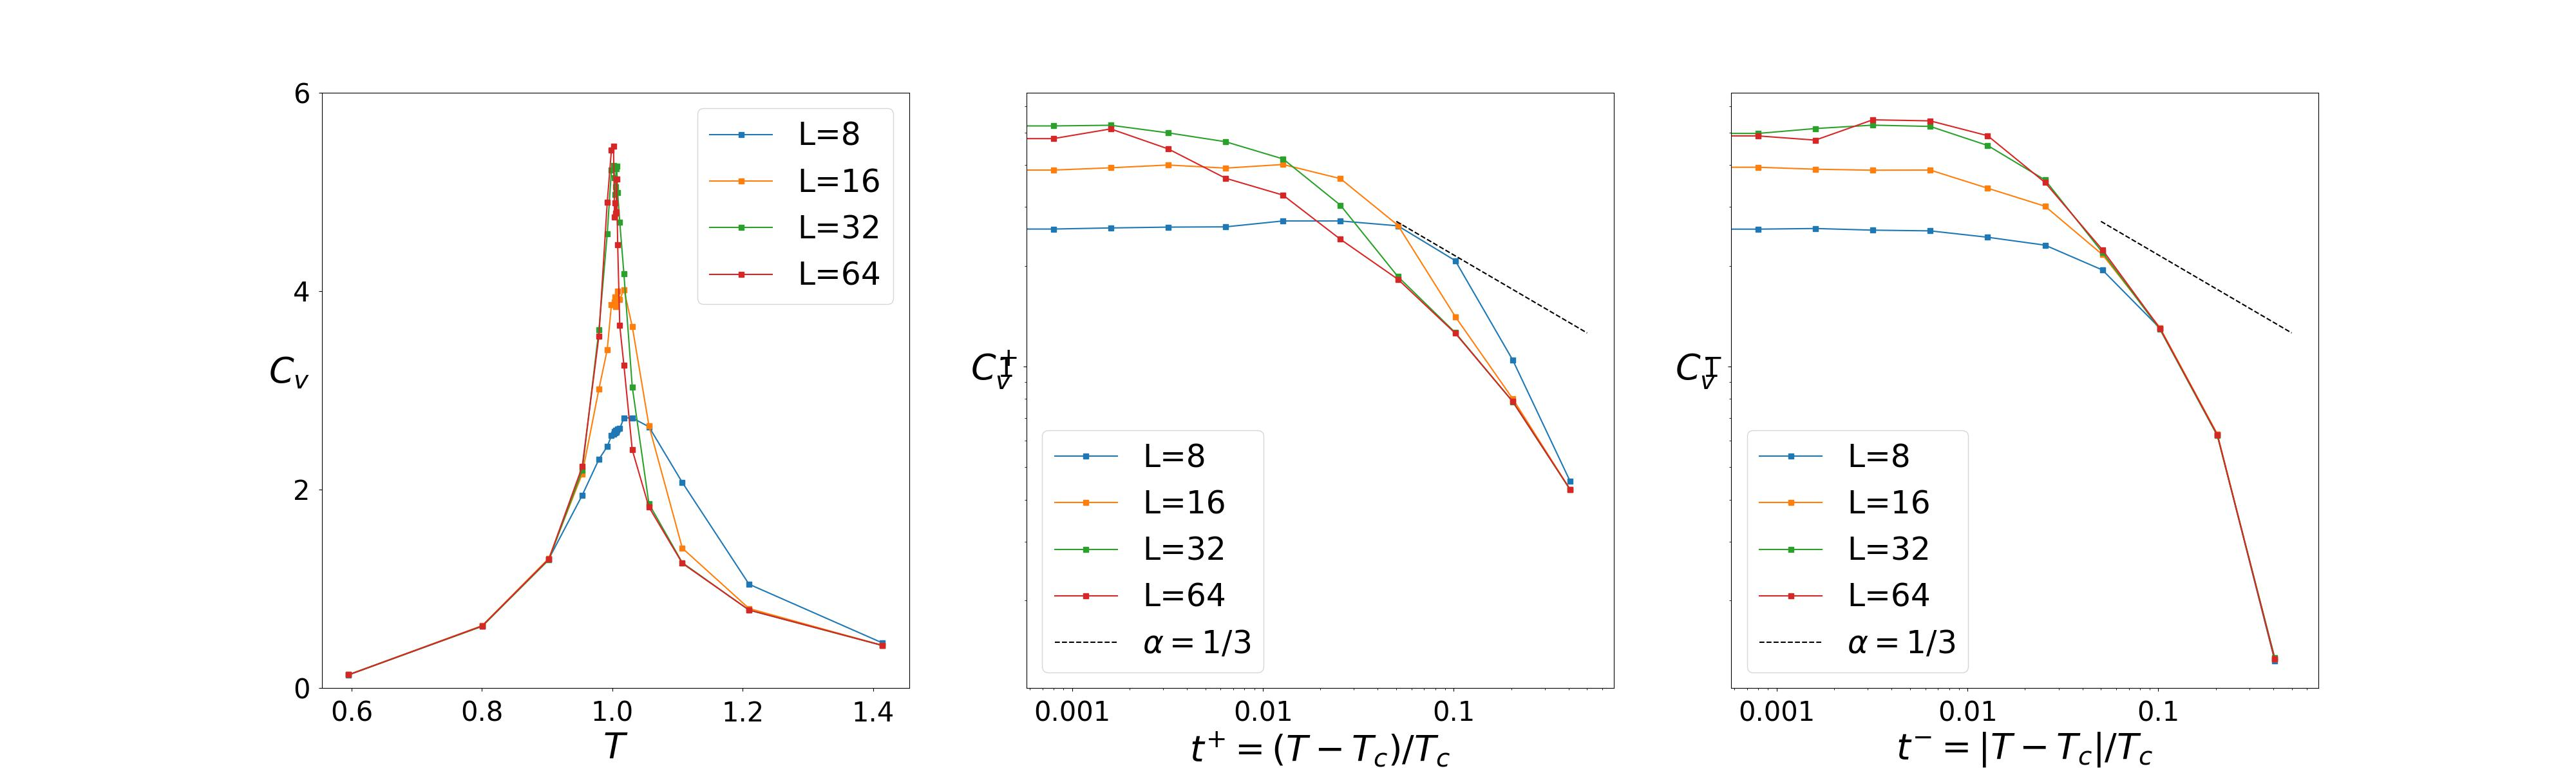
\includegraphics[width=1\textwidth]{../fig/Alpha, Specific Heat (3-state 2D Potts).jpg}
\caption{\label{fig:alpha} Specific Heat $C_{v}$ of the system at Size = 8, 16, 32, 
and 64. $\alpha = 1/3$}
\end{figure*}

\begin{figure*}[b]
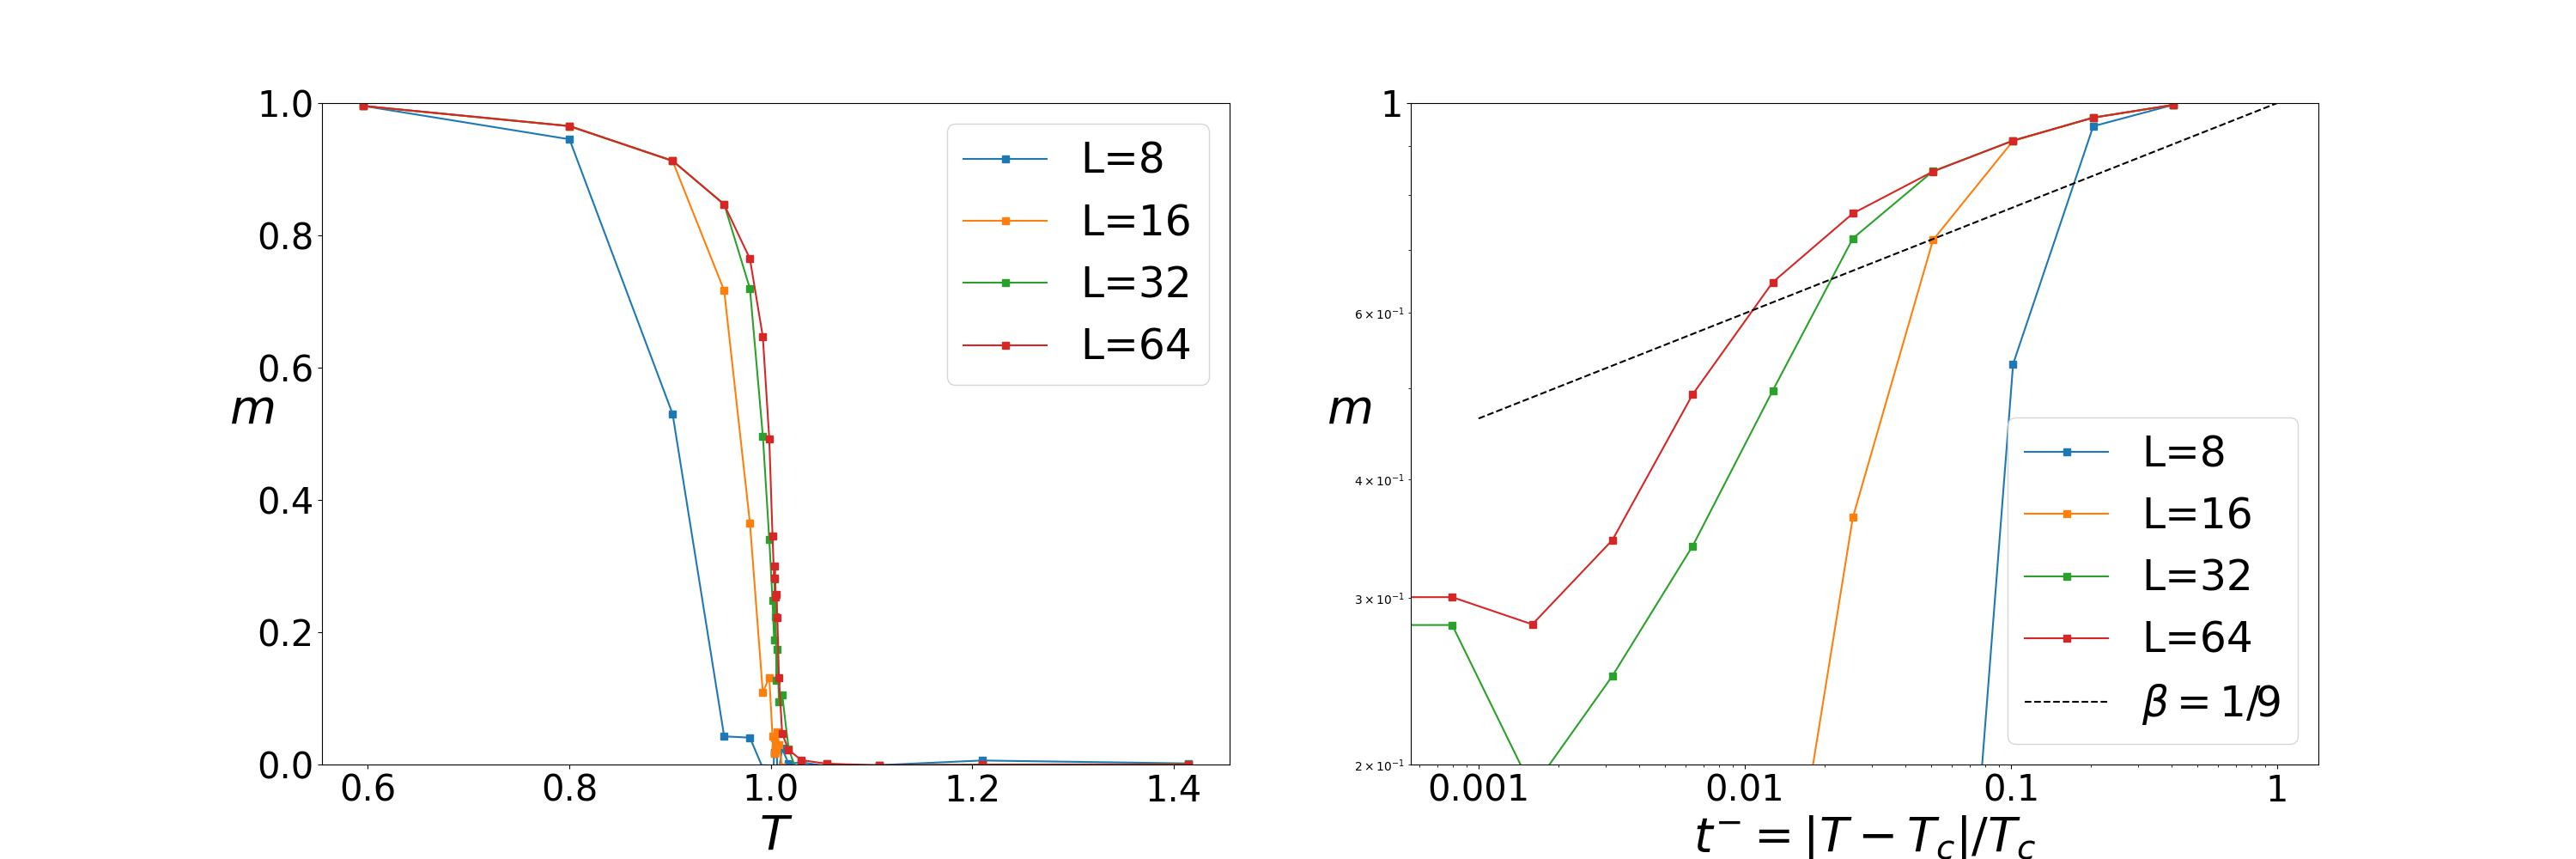
\includegraphics[width=0.9\textwidth]{../fig/Beta, Order Parameter (3-state 2D Potts).jpg}
\caption{\label{fig:beta} Order Parameter $m$ of the system with no external field 
at Size = 8, 16, 32, and 64. $\beta = 1/9$}
\end{figure*}

\begin{figure*}[b]
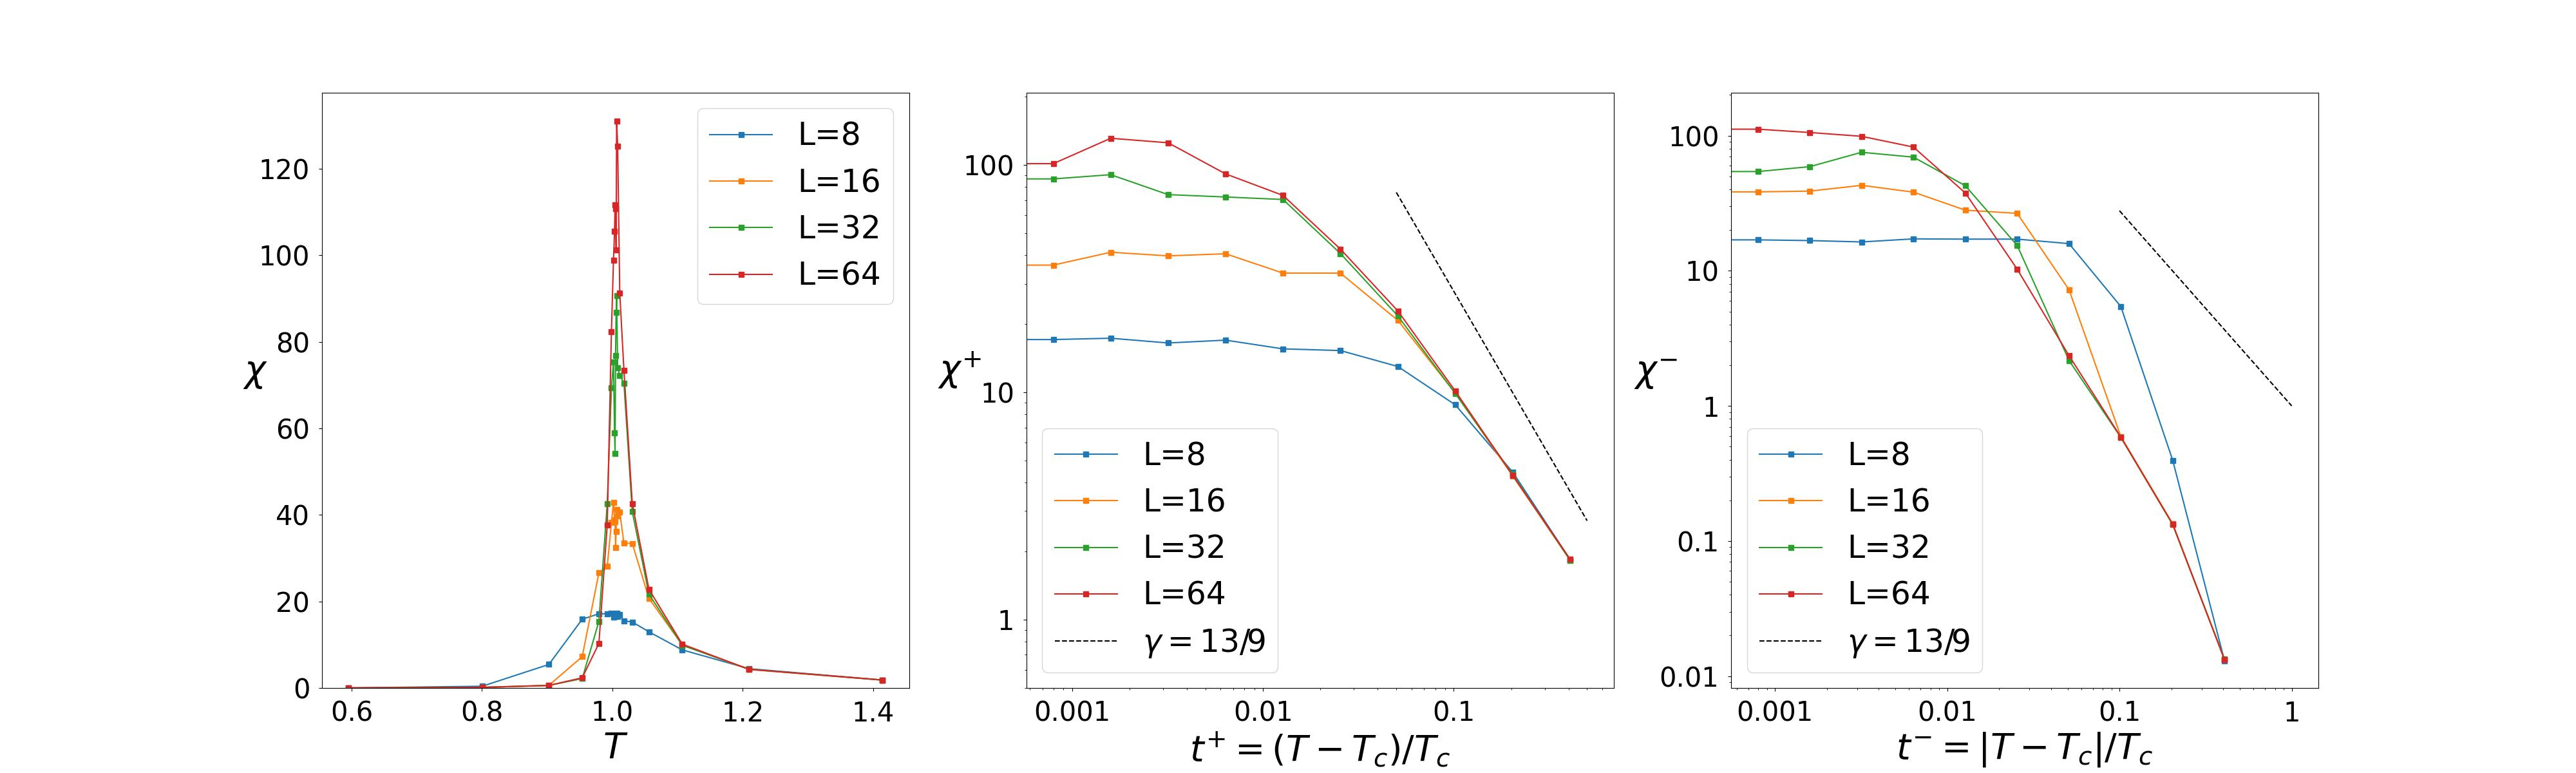
\includegraphics[width=1\textwidth]{../fig/Gamma, Susceptibility (3-state 2D Potts).jpg}
\caption{\label{fig:gamma} Susceptibility $X_{T}$ of the system at Size = 8, 16, 32, 
and 64. $\gamma = 13/9$}
\end{figure*}

\begin{figure*}[b]
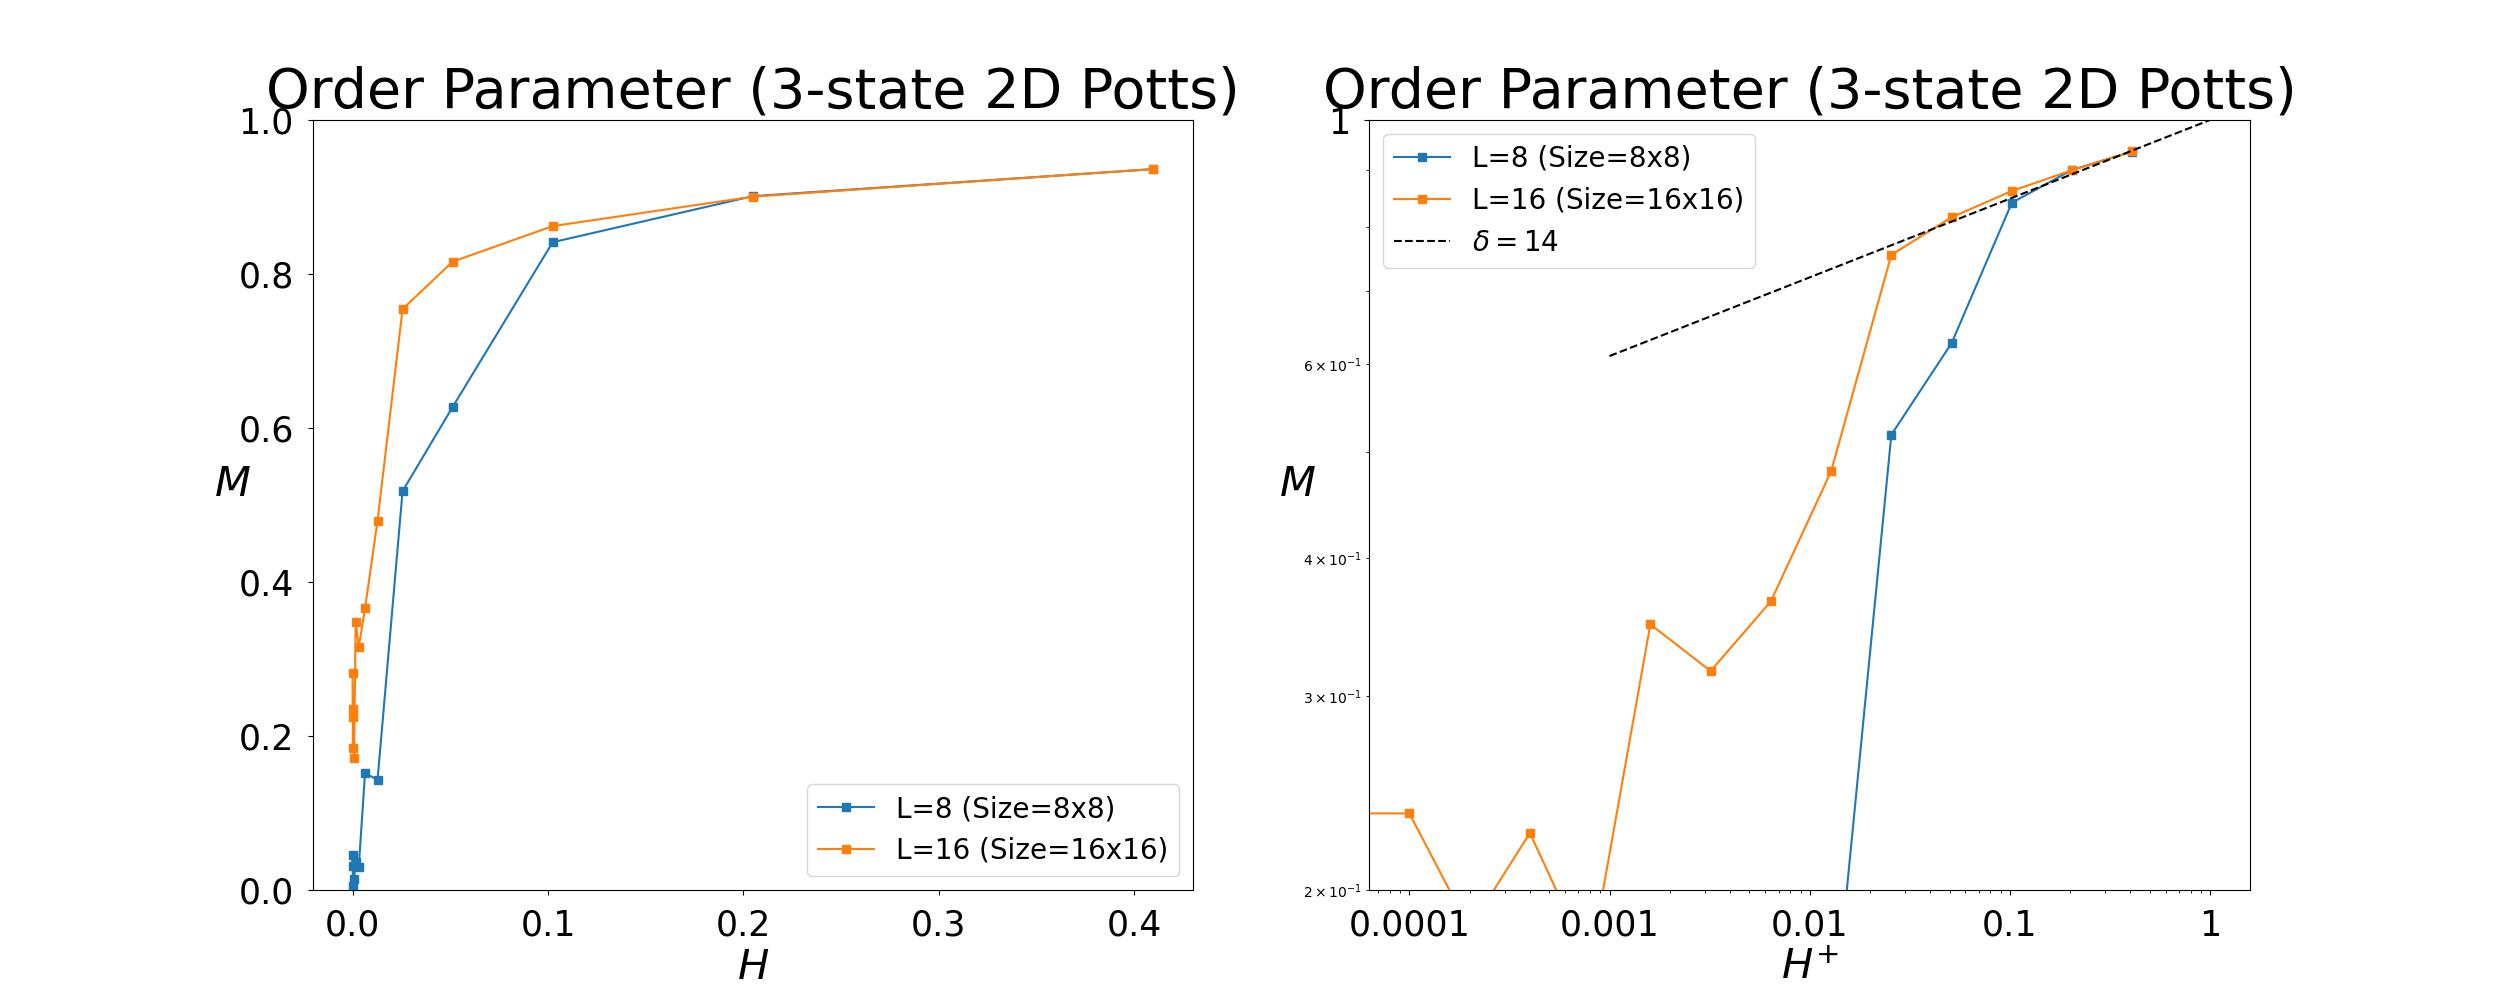
\includegraphics[width=0.8\textwidth]{../fig/Delta, Order Parameter (3-state 2D Potts).jpg}
\caption{\label{fig:delta} Order Parameter $m$ of the system at $t=0$ at Size = 8, 16, 32, 
and 64. $\delta = 14$}
\end{figure*}

\begin{figure*}[b]
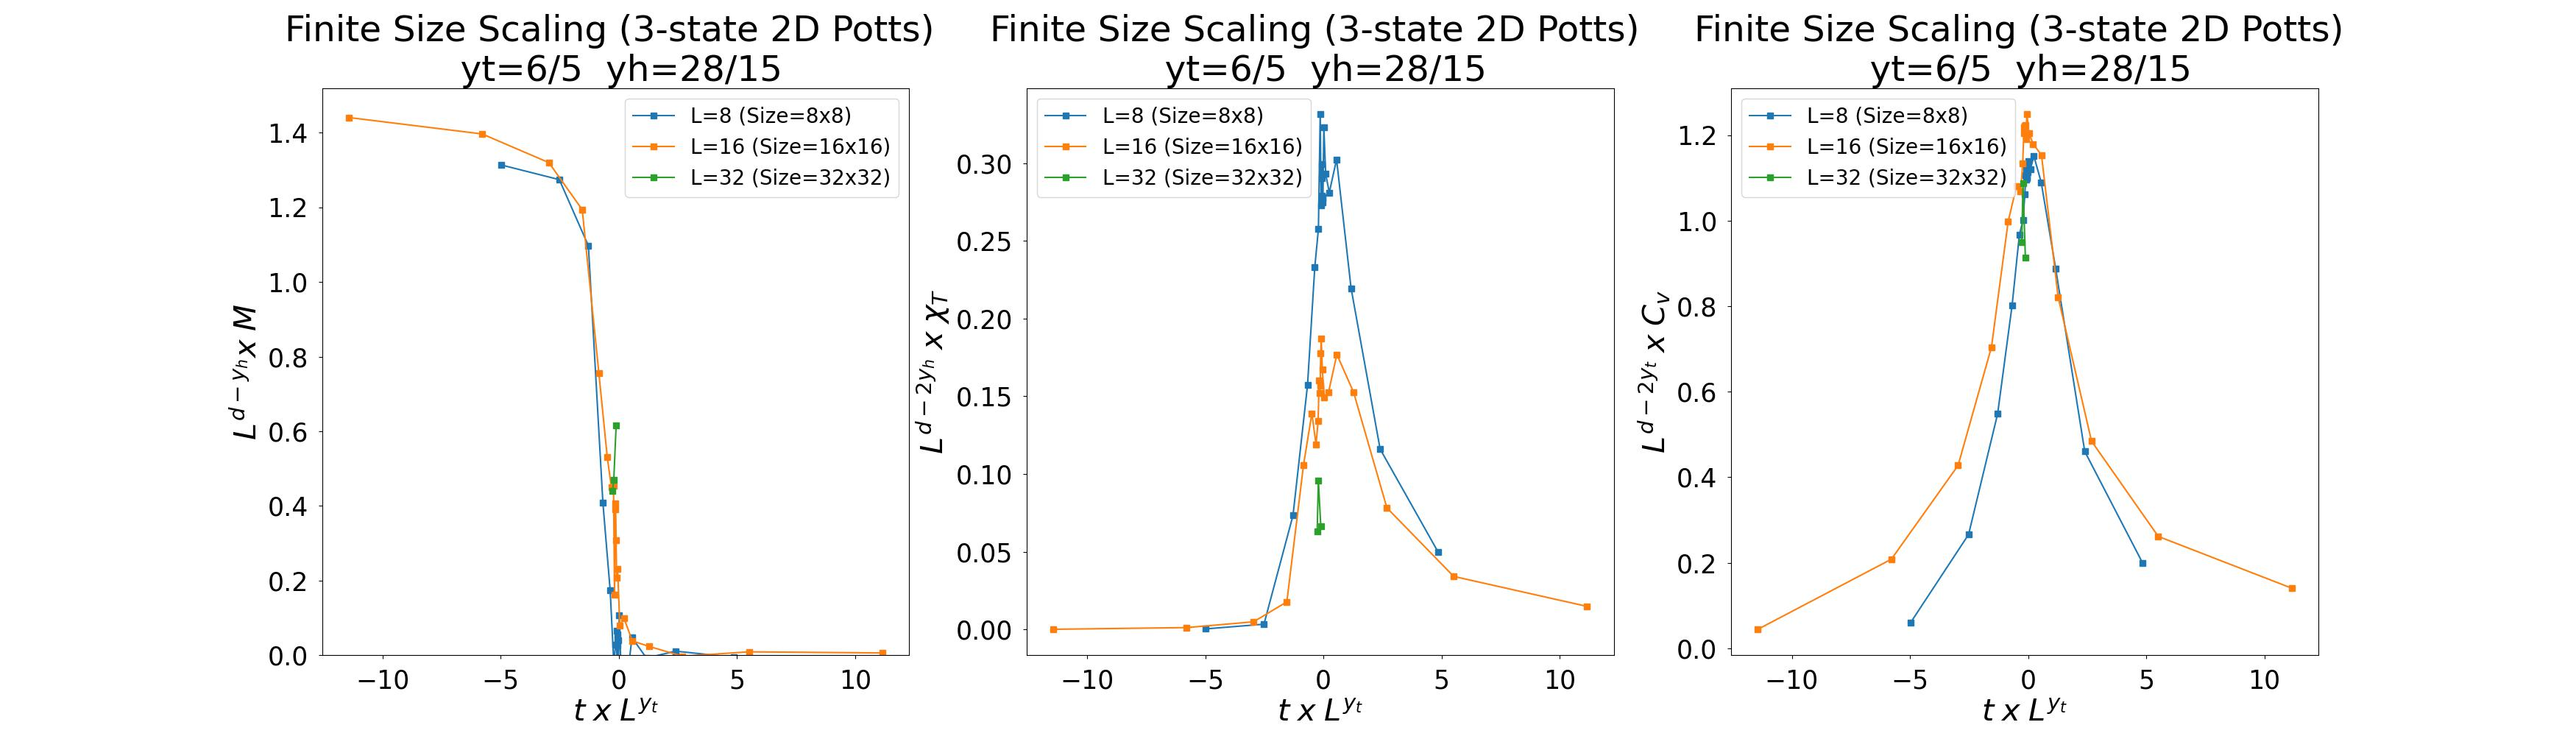
\includegraphics[width=1\textwidth]{../fig/Finite Size Scaling (3-state 2D Potts).jpg}
\caption{\label{fig:fss} Finite Size Scaling of the system at Size = 8, 16, 32, and 64. 
$y_{t} = 6/5 \text{ and } y_{h} = 28/15$}
\end{figure*}

\begin{figure*}[b]
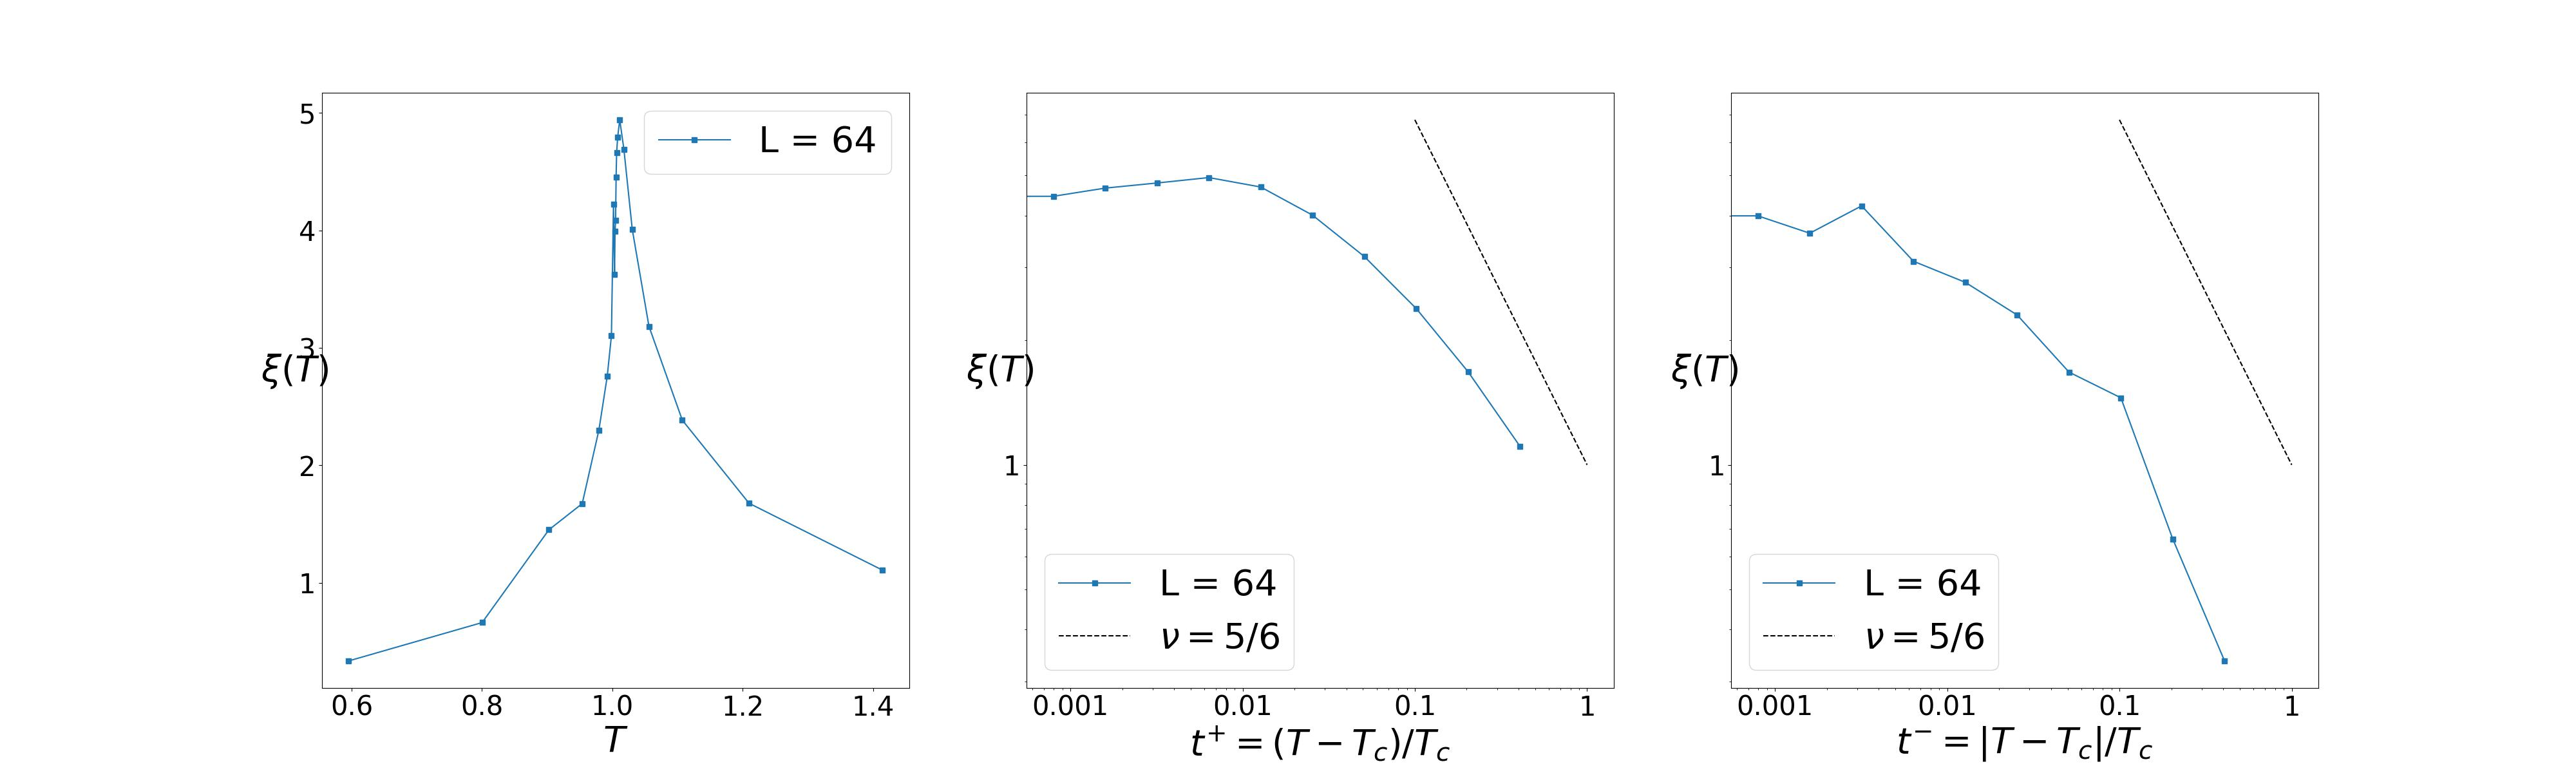
\includegraphics[width=1\textwidth]{../fig/Correlation Length (3-state 2D Potts).jpg}
\caption{\label{fig:corrlength} Correlation Length $\xi$ of the system at Size = 64. 
$\nu = 5/6$}
\end{figure*}

\begin{figure}[b]
\includegraphics[width=0.5\textwidth]{../fig/Correlation Function (3-state 2D Critical 
Potts).jpg}
\caption{\label{fig:corrfunc} Correlation Function $G(i,j)$ of the system at critical 
fixed point at Size = 8, 16, 32, and 64. $\eta = 4/15 \text{ since } d = 2$}
\end{figure}

\section{\label{sec:rsrg}Theoretical Method 1: \\ Real-Space Renormalization Group}
In this section, we calculate the coupling exponents of 3-state Potts model in 2 dimension 
by utilizing Block-Spin Transformation technique, a well-known analytic realization in 
Real-space Renormalization Group. To avoid further complication, we will be applying this 
technique to the Potts model on triangular lattice since the topological aspect of the
lattice, unlike the dimension, has no affect on the value of coupling exponents. \\

As sdisplayed in Fig.~\ref{fig:tri}, we first group sites on the triangular lattice into 
triples on triangles and then coarse grain the system b choosing a representative single 
spin value for each of the triples forming a new triangular lattice with scale factor 
$b=\sqrt 3$. \\

\begin{figure}[b]
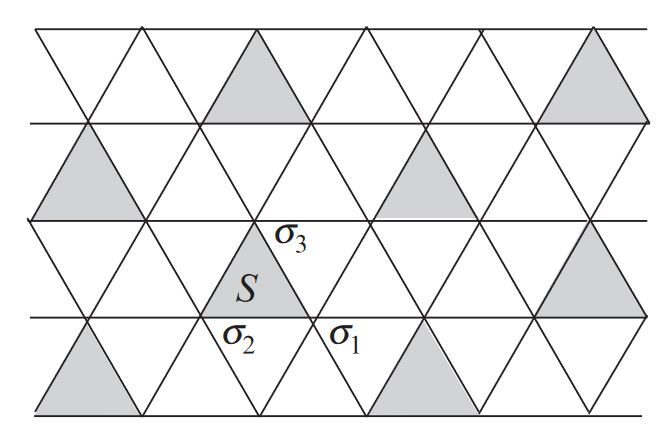
\includegraphics[width=0.4\textwidth]{../fig/triangular lattice.JPG}
\caption{\label{fig:tri} Three spins on a shaded triangle $\sigma_{1}, \sigma_{2}, 
\text{ and } \sigma_{3}$ are grouped into a scaled block spin $S$ with value determined
by the majority rule.}
\end{figure}

For newly denoted block spin $S$ grouped from $\sigma_{1}, \sigma_{2}, \text{ and } 
\sigma_{3}$, the value are assigned in accordance to the majority rule. For $\sigma$
spin configuration $\sigma_{I} = \{\sigma_{1}\sigma_{2}\sigma_{3}\}$ in block lattice $I$, 
the block spin $S_{I}$ that forms the coarsed-grain system is transformed as

\begin{gather}
\{000, 001, 010, 100, 002, 020, 200, (012) \} \rightarrow S_{I}=0 \\
\{111, 110, 101, 011, 112, 121, 211, (012) \} \rightarrow S_{I}=1 \\
\{222, 220, 202, 022, 221, 212, 122, (012) \} \rightarrow S_{I}=2
\end{gather}

where for configuration $\{012\}$, the block spin is assigned randomly with equal 
probability. \\

The block-spin $S$ forms a new Hamiltonian $H'$ scaled from the original Hamiltonian $H$.

\begin{gather}
H = -K\sum_{\left<i,j\right>}\delta(\sigma_{i}, \sigma_{j}) -h\sum_{i}\delta(\sigma_{i},0) \\
H'= -K'\sum_{\left<I,J\right>}\delta(S_{I}, S_{J}) -h'\sum_{I}\delta(S_{I},0) \label{eqn:Hpri}
\end{gather}

The coupling exponent $y_t \text{ and } y_h$ is given as a derivative betweem original and 
scaled coupling parameter $K, h$ and $K'(K,h), \text{ } h'(K,h)$.

\begin{eqnarray}
b^{y_{t}} = \frac{\partial K'}{\partial K}\bigg|_{K_c,h_c} \text{ and } 
b^{y_{h}} = \frac{\partial h'}{\partial h}\bigg|_{K_c,h_c} \label{eqn:exp}
\end{eqnarray}

Therefore, our goal is to calculate the scaled coupling parameter $K' \text{ and } h'$ from
the following relation which is a combination of Eq.~(\ref{eqn:newHam}) and~(\ref{eqn:Hpri}).

\begin{gather}
\sum_{\{S\}}e^{K'\sum_{\left<I,J\right>}\delta(S_{I}, S_{J}) +h'\sum_{I}\delta(S_{I},0)} = 
\sum_{\{\sigma\}}e^{-H} \\
H' = -\ln\left[\sum_{\{\sigma^{S}\}} e^{K\sum_{\left<i,j\right>}\delta(\sigma_{i}, \sigma_{j}) 
+h\sum_{i}\delta(\sigma_{i},0)}\right] \label{eqn:block-spin}
\end{gather}

where the term $\{\sigma^{S}\}$ represents the set of spin configuration $\sigma$ when 
$S$ is given. \\

The RHS of Eq.~(\ref{eqn:block-spin}) can be elaborated as follows to obtain a useful version of the 
renormalization group equation that describes the flow.

\begin{widetext}
\begin{gather}
\sum_{\{\sigma^{S}\}} e^{K\sum_{\left<i,j\right>}\delta(\sigma_{i}, \sigma_{j}) 
+h\sum_{i}\delta(\sigma_{i},0)}
= \sum_{\{\sigma^{S}\}} e^{K\sum_{\left<i,j\in I\right>}\delta(\sigma_{i}, \sigma_{j}) 
+h\sum_{i}\delta(\sigma_{i},0) + K\sum_{\left<i\in I, j \in J\right>}\delta(\sigma_{i}, 
\sigma_{j})} \\
= \sum_{\{\sigma^{S}\}} e^{K\sum_{\left<i,j\in I\right>}\delta(\sigma_{i}, \sigma_{j}) 
+h\sum_{i}\delta(\sigma_{i},0)} \times \frac{\sum_{\{\sigma^{S}\}} e^{K\sum_{\left<i,j\in 
I\right>}\delta(\sigma_{i}, \sigma_{j}) +h\sum_{i}\delta(\sigma_{i},0)} 
\times e^{K\sum_{\left<i\in I, j \in J\right>}\delta(\sigma_{i}, \sigma_{j})}}
{\sum_{\{\sigma^{S}\}} e^{K\sum_{\left<i,j\in I\right>}\delta(\sigma_{i}, \sigma_{j}) 
+h\sum_{i}\delta(\sigma_{i},0)}} \\
= \sum_{\{\sigma^{S}\}} e^{-H_{0}} \times \frac{\sum_{\{\sigma^{S}\}} e^{-H_{0}} \times 
e^{-V}}{\sum_{\{\sigma^{S}\}} e^{-H_{0}}}
= \prod_{I} Z_{\text{block}} \times \left<e^{-V}\right>_{0}
= \prod_{I} Z_{\text{block}} \times \left<e^{K\sum_{\left<i\in I, j \in J\right>}
\delta(\sigma_{i}, \sigma_{j})}\right>_{0}
\end{gather}

\begin{gather}
K'\sum_{\left<I,J\right>}\delta(S_{I}, S_{J}) + h'\sum_{I}\delta(S_{I},0) 
= \sum_{I} \ln\left[Z_{\text{block}}\right] + \ln\left[\left<e^{K\sum_{\left<i \in I, 
j \in J\right>} \delta(\sigma_{i}, \sigma_{j})}\right>_{0}\right] \\
\approx \sum_{I} \ln\left[Z_{\text{block}}\right] + \left<K\sum_{\left<i \in I, 
j \in J\right>} \delta(\sigma_{i}, \sigma_{j})\right>_{0} + \dotsb
\approx \sum_{I} \ln\left[Z_{\text{block}}\right] + K \sum_{\left<I,J\right>} 
\left<\delta(\sigma_{I1}, \sigma_{J2}) + \delta(\sigma_{I3}, \sigma_{J2})\right>_{0} \\
\approx \sum_{I} \ln\left[Z_{\text{block}}\right] + 2K \sum_{\left<I,J\right>} 
\left<\delta(\sigma_{I1},\sigma_{J2})\right>_{0} \\
\approx \sum_{I} \ln\left[Z_{\text{block}}\right] + 2K \sum_{\left<I,J\right>} \big[
\left<\delta(\sigma_{I1},0)\right>_{0}\left<\delta(\sigma_{J2},0)\right>_{0} + 
\left<\delta(\sigma_{I1},1)\right>_{0}\left<\delta(\sigma_{J2},1)\right>_{0} + 
\left<\delta(\sigma_{I1},2)\right>_{0}\left<\delta(\sigma_{J2},2)\right>_{0}\big] 
\end{gather}
\end{widetext}

While $\left<\dotsb\right>_{0}$ is the expectation value with respect to the weight of 
internal block Hamiltonian $H_{0}$. Fig~\ref{fig:intra} shows the inter-block relation 
between block indices $I=1 \text{ and } J=2$, note that in triangular lattice, 
there are 6 nearest-neighbor indices after block-spin transformation. \\

\begin{figure}[b]
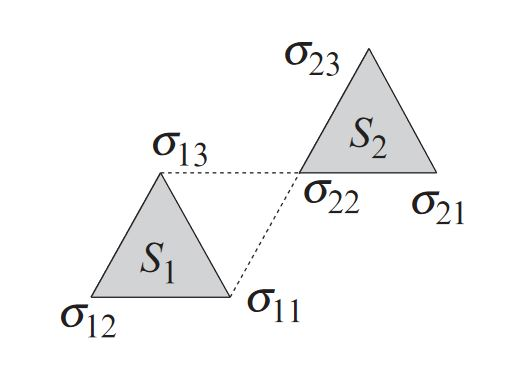
\includegraphics[width=0.4\textwidth]{../fig/effective interblock interaction.JPG}
\caption{\label{fig:intra} Inter-block relation between block indices $I=1 \text{ and } J=2$.
It is worth mentioning that in triangular lattice, there are 6 nearest-neighbor indices 
after block-spin transformation.}
\end{figure}

If we denote $Z_{\text{block}} = \exp[C_{1} + D \delta(S_{I},0)]$ and 
$\left<\delta(\sigma_{I1},\sigma_{J2})\right>_{0} = A\delta(S_{I},S_{J}) + 
B\delta(S_{I},0) + B\delta(S_{J},0) + C_{2}$, the renormalization group equation is 
written as

\begin{gather}
K' = 2KA(K,h) \label{eqn:rgeq1}\\
h' = D(K,h) + 6 \times 2KB(K,h) \label{eqn:rgeq2}
\end{gather}

Explicit calculations through majority rule and rescaling in triangular lattice
reveals the following result.

\begin{align}
A(K,h) = \left(\frac{e^{3K}+2e^{K+h}+e^{K}}{e^{3K}+3e^{K+h}+3e^{K}+2e^{h}}\right)^{2}
\end{align}

\begin{widetext}
\begin{multline}
B(K,h) = \frac{1}{2} \times \Bigg[
\frac{\left(e^{3K+3h}+4e^{K+2h}+2/3e^{h}\right)^2 + 2\left(e^{K+2h}+2/3e^{h}\right)^2}
{\left(e^{3K+3h}+6e^{K+2h}+2e^{h}\right)^2}\\ 
- \frac{\left(e^{3K}+2e^{K+h}+2e^{K}+2/3e^{h}\right)^2+\left(e^{K+h}+2/3e^{h}\right)^2+
\left(e^{K}+2/3e^{h}\right)^2}
{\left(e^{3K}+3e^{K+h}+3e^{K}+2e^{h}\right)^2} \Bigg]
\end{multline}
\end{widetext}

% \begin{widetext}
% \begin{multline}
% p(x) = 3x^6 + 14x^5y + 590x^4y^2 + 19x^3y^3\\ 
% - 12x^2y^4 - 12xy^5 + 2y^6 - a^3b^3
% \end{multline}
% \end{widetext}

\begin{align}
D(K,h) = \ln\left[\frac{e^{3K+3h}+6e^{K+2h}+2e^{h}}{e^{3K}+3e^{K+h}+3e^{K}+2e^{h}}\right]
\end{align}

One can determine the critical fixed point with infinite correlation length by applying
$K=K'=K_c \text{ and }h=h'=h_c$ in Eq.~(\ref{eqn:rgeq1}) and~(\ref{eqn:rgeq2}).

\begin{eqnarray}
\left(K_c,h_c\right) = (0.911, 0) \label{eqn:cfp}
\end{eqnarray}

As a result, the coupling parameter for temperature and external magnetic field is

\begin{gather}
y_{t} = \ln\left[\frac{\partial K'}{\partial K} \bigg|_{(0.911,\text{ }0)}\right] / \ln\sqrt3 = 1.102 \\
y_{h} = \ln\left[\frac{\partial h'}{\partial h} \bigg|_{(0.911,\text{ }0)}\right] / \ln\sqrt3 = 2(?)
\end{gather}

which is pretty close to the exact value of $(6/5, \text{ } 28/15)$ for 3-state Potts model 
in 2 dimension.

\section{\label{sec:mcrg}Numerical Method 2: \\ Monte Carlo Renormalization Group}
Monte Carlo Renormalization Group (MCRG) is a numerical method used to study the 
behavior of statistical systems in physics and related fields. It is based on the 
idea of the Renormalization Group, but instead of analytically solving flow equations, 
MCRG uses computer simulations to generate a sequence of approximate solutions for 
the system under consideration. \\

In MCRG, the system is treated as a set of discrete variables, and the values of 
these variables are updated using a random process based on the Metropolis algorithm. 
The updates are performed repeatedly, and the resulting configurations are used to 
calculate various properties of the system. Over time, the RG transformation is carried 
out by changing the scale at which the system is studied, leading to the creation of a 
block-spin representation that summarizes the behavior of the system at different scales.\\

MCRG is commonly used in computational physics and is considered a powerful tool for 
studying complex systems, especially those that exhibit phase transitions or 
critical phenomena. \\

TBA

\section{\label{sec:cft}Theoretical Method 2: \\ Conformal Field Theory}
Conformal field theory (CFT) is a type of field theory that is characterized by the 
presence of conformal symmetry, which is a set of transformations that preserve angles 
and ratios of distances in a two-dimensional space. Conformal symmetries are important 
in many areas of physics and mathematics, including string theory, condensed matter 
physics, and statistical mechanics. \\

The Virasoro algebra is a Lie algebra that plays a central role in conformal field theory. 
It is a symmetry algebra of the conformal group, which is the group of transformations that 
preserve conformal symmetry. The Virasoro algebra is generated by a set of 
infinite-dimensional operators, known as Virasoro generators, which encode the symmetries 
of the theory and describe the behavior of the theory under conformal transformations. \\

The Virasoro algebra is used to classify and study the symmetries of conformal 
field theories, and it is an important tool in the study of critical phenomena, 
such as phase transitions. In particular, it provides a way to study the behavior of 
two-dimensional field theories under scale transformations, which are important in 
understanding the critical behavior of systems near a phase transition. \\

The representation of Virasoro Algebra describes the basis of conformal field theory in 2 
dimension. For coprime integers $p, q \geq 2 \text{ and } r=1\sim q-1, s=1\sim p-1$,

\begin{gather}
c_{p,q} = 1-\frac{6(p-q)^2}{pq} \\
h_{r,s} = \frac{(pr-qs)^2-(p-q)^2}{4pq}
\end{gather}

where $c_{p,q} \text{ and } h_{r,s}$ is a central charge and conformal weight of the system, 
respectively. It is worth noting that the total number of primary fields is $(p-1)(q-1)/2$.\\

The representation is unitary if and only if $|p-q|=1$, e.g. $p=m+1 \text{ and }q = m$.

\begin{gather}
c=1-\frac{6}{m(m+1)} \text{ for m=3,4,5} \dotsb \\
h_{r,s} = \frac{\left[(m+1)r-ms\right]^2-1}{4m(m+1)}
\end{gather}

The critical ising model in 2 dimension is represented by $m=3$ while the conformal symmetry 
of critical 3-state Potts model in 2 dimension is described by the unitary representation 
of Virasoro Algebra with $m=5$. One can calculate the temperature and magnetic coupling 
exponents from their respective conformal weights associated with the primary fields.

\begin{gather}
y_{t} = 2 - 2h_{2,1} = 2 - \frac{4}{5} = \frac{6}{5} \\
y_{h} = 2 - 2h_{2,3} = 2 - \frac{2}{15} = \frac{28}{15}
\end{gather}

TBA

\section{Conclusions}
Conclusion.

% \paragraph{Syntax}

\begin{acknowledgments}
The code that generates data for Finite Size Scaling in Section~\ref{sec:fss} in this paper
is available at https://github.com/LEE-SungBin/potts.git.
\end{acknowledgments}

\appendix

\section{\label{appx:fluc}Fluctuation-dissipation theorem}
Consider an arbitrary system whose Hamiltonian $H(0)$ is modified because of the presence of 
an external inhomogeneous field $B(r)$ as

\begin{eqnarray}
H = H_{0} -\int dr O(r)B(r)
\end{eqnarray}

where $O(r)$ is the system variable that linearly couples to the external field. The free 
energy $F = -\beta^{-1} \ln Z$ in terms of the partition function

\begin{eqnarray}
Z = \Tr\left[\exp\left(-\beta H_{0} + \beta \int dr O(r)B(r)\right)\right]
\end{eqnarray}

The generalized isothermal susceptibility is defined as follows:

\begin{eqnarray}
\chi(r,r') := -\frac{\partial^2 F}{\partial B(r) \partial B(r')}
\end{eqnarray}

as the second-order functional derivative of the free energy with the result

\begin{multline}
\chi(r,r') = \beta^{-1} \bigg[\frac{1}{Z} \frac{\partial^2 Z}{\partial B(r) \partial B(r')} \\
-\frac{1}{Z}\frac{\partial Z}{\partial B(r)} \frac{1}{Z} \frac{\partial Z}{\partial B(r')} \bigg]
\end{multline}

Therefore, the generalized isothermal susceptibility is proportional to the correlation 
function between two corresponding points.

\begin{multline}
\chi(r,r') = \beta G(r,r') \\
= \beta \left[\left<O(r)O(r')\right>-\left<O(r)\right>\left<O(r')\right>\right]
\end{multline}

If the system is translation invariant, we can sum over the both hand side to get the 
fluctuation-dissipation theorem.

\begin{eqnarray}
\chi = \int dr \chi(r) = \beta \int dr G(r)
\end{eqnarray}

\section{\label{appx:rsrg-ising}Real-Space Renormalization Group for Ising Model on 
two dimensional square lattice}
Real-space Renormalization Group for Ising Model on two dimensional square lattice is more 
or less similiar to that for the 3-state Potts model. The block-spin transformation satisfies
the following majority principle for spin $\sigma = \pm 1$.

\begin{gather}
\{++++,\overline{+++-},\widehat{++--},\widehat{+-+-}\} \rightarrow S_{I} = + \\
\{----,\overline{---+},\widehat{--++},\widehat{-+-+}\} \rightarrow S_{I} = -
\end{gather}

The renormalization group equation for ising model is given as

\begin{widetext}
\begin{gather}
K'\sum_{\left<I,J\right>}S_{I}S_{J}+h'\sum_{I}S_{I} \approx 
\sum_{I} \ln\left[Z_{\text{block}}\right] + 2K \sum_{\left<I,J\right>}
\left<\sigma_{I4}\right>_{0}\left<\sigma_{J1}\right>_{0}
\end{gather}
\end{widetext}

If we set $Z_{\text{block}} = \exp[C+DS_{I}]$ and $\left<\sigma_{I4}\right>_{0} = A + BS_{I}$,
The renormalization equation is simplified as follows:

\begin{gather}
K' = 2KB(K,h)^{2} \\
h' = D(K,h) + 4 \times 2KA(K,h)B(K,h)
\end{gather}

After some calculation, it is straight forward to prove

\begin{multline}
A(K,h) = \frac{1}{2} \bigg[\frac{e^{4K+4h}+2e^{2h}}{e^{4K+4h}+4e^{2h}+2+e^{-4K}} \\
- \frac{e^{4K-4h}+2e^{-2h}}{e^{4K-4h}+4e^{-2h}+2+e^{-4K}}\bigg]
\end{multline}
\begin{multline}
B(K,h) = \frac{1}{2} \bigg[\frac{e^{4K+4h}+2e^{2h}}{e^{4K+4h}+4e^{2h}+2+e^{-4K}} \\
+ \frac{e^{4K-4h}+2e^{-2h}}{e^{4K-4h}+4e^{-2h}+2+e^{-4K}}\bigg]
\end{multline}
\begin{gather}
D(K,h) = \ln\left[\frac{e^{4K+4h}+4e^{2h}+2+e^{-4K}}{e^{4K-4h}+4e^{-2h}+2+e^{-4K}}\right]
\end{gather}

Therefore, we can theoretically derive the critical fixed point and temperature and magnetix
exponent of the ising model in 2 dimension.

\begin{gather}
\left(K_{c}, h_{c}\right) = (0.5, 0)
\end{gather}

Note that the exact critical temperature of ising model in 2 dimensional square lattice is
$K_{c} = \frac{\ln\left[1+\sqrt2\right]}{2} = 0.441$.

\begin{gather}
y_{t} = \ln\left[\frac{\partial K'}{\partial K} \bigg|_{(0.5,0)}\right] / \ln2 =  \\
y_{h} = \ln\left[\frac{\partial h'}{\partial h} \bigg|_{(0.5,0)}\right] / \ln2 = 
\end{gather}

which is pretty close to the exact value of $(1, \text{ } 15/8)$ for Ising model 
in 2 dimension.\\

\section{\label{appx:universal}Universality Class}
Universality Class is a set of physical system that shares an identical scale invariant 
limit under the process of renormalization group flow. While the model may seem to evolve 
in time differently in most situations, their behavior will converge to a certain 
classification as they reach the scale limit. \\

The most prominent examples of the universality class is the critical exponents of the 
system which describes the asymptotic phenomena of the model as they approach the phase 
transition point. Table~\ref{tab:universality} and~\ref{tab:exponent} shows the full list 
of critical exponents and critical coupling exponents for several well-known physical 
system that exhibit critical phenomena or phase transitions. \\ 

\begin{table}[b]
\caption{\label{tab:universality}
A full list of critical exponents of various physical systems that shows phase transition. 
Each critical exponents describes the asymptotic behavior of the physical quantities as the 
system approaches phase transition.}
\begin{ruledtabular}
\begin{tabular}{cccccccc}
Class &$d$ &$\alpha$ &$\beta $&$\gamma $&
$\delta$ &$\nu$ &$\eta$ \\
\hline
Ising & 2 & 0 & 1/8 & 7/4
& 15 & 1 & 1/4 \\
Ising & 3 & 0.11 & 0.33 & 1.24
& 4.79 & 0.63 & 0.04 \\
3-state Potts & 2 & 1/3 & 1/9 & 13/9
& 14 & 5/6 & 4/15 \\
4-state Potts & 2 & 2/3 & 1/12 & 7/6
& 15 & 2/3 & 1/4 \\
XY & 3 & -0.02 & 0.35 & 1.32
& 4.78 & 0.67 & 0.04 \\
Heisenberg & 3 & -0.12 & 0.37 & 1.40
& 4.78 & 0.71 & 0.04 \\
Mean Field &  & 0 & 1/2 & 1
& 3 & 1/2 & 0 \\
\end{tabular}
\end{ruledtabular}
\end{table}

\begin{table}[b]
\caption{\label{tab:exponent}
A full list of critical temperature and external field exponents of various physical system 
that shows phase transition. It is worth noting that every critical exponents which 
describes the asymptotic behavior of physical system near critical point can be calculated
from the coupling parameter via scaling relations.}
\begin{ruledtabular}
\begin{tabular}{cccccccc}
Class &$d$ &$y_{t}$ &$y_{h}$\\
\hline
Ising & 2 & 1 & 15/8 \\
Ising & 3 & 1.59 & 2.48 \\
3-state Potts & 2 & 6/5 & 28/15 \\
4-state Potts & 2 & 3/2 & 15/8 \\
XY & 3 & 1.49 & 2.48 \\
Heisenberg & 3 & 1.41 & 2.48 \\
\end{tabular}
\end{ruledtabular}
\end{table}

% The \nocite command causes all entries in a bibliography to be printed out
% whether or not they are actually referenced in the text. This is appropriate
% for the sample file to show the different styles of references, but authors
% most likely will not want to use it.
% \nocite{*}
% \bibliographystyle{abbrv}
% \bibliography{../ref/ref} % Produces the bibliography via BibTeX.

\end{document}
%
% ****** End of file apssamp.tex ******
